\section{Twin Contacts}
A twin test must require two heights to vanish simultaneously. Their
difference is unsuitable: it vanishes whenever the heights agree, including
when both are positive. For example, $h(8)=h(10)=2$, although neither
endpoint is prime. Nonnegativity makes their sum the appropriate condition.

\begin{itemize}
\item Pair waves built from the same endpoint filters.
\item Exact twin contacts and finite-stage certification.
\end{itemize}

For integer $M\ge1$ and real $t\ge2$, define
\begin{equation*}
\begin{aligned}
B_M(t)&=h_M(t)+h_M(t+2),\\
T_M(t)&=t+i B_M(t),\\
V_m(t)&=a_m(t)W_m(t)+a_m(t+2)W_m(t+2)\quad(m\ge2).
\end{aligned}
\end{equation*}

This uses the same wave at both endpoints. There is no separate prime
generator inside the pair construction. Since $\sin^2(\pi(t+2))=\sin^2(\pi t)$,
substitution gives
\begin{equation*}
\begin{aligned}
B_M(t)&=2\sin^2(\pi t)+\sum_{m=2}^{M}V_m(t)
&&[\text{By Definition}]\\
T_M(t)&=T_{M-1}(t)+i V_M(t)\quad(M\ge2).
&&[\text{Subtraction}]
\end{aligned}
\end{equation*}

The real coordinate remains the pair's starting value $t$. Adding $F_M(t)$
and $F_M(t+2)$ directly would change that coordinate to $2t+2$.

Each endpoint is protected according to its own argument. The new pair
contribution vanishes when $t+2\le M$, but may change a start $t\le M$
whose second endpoint lies beyond $M$. This explains why preserving the
past for the single curve and for the pair curve requires different cutoffs.

For a bounded interval of starts $[2,X]$, both endpoint heights are fully
stabilized once $M\ge\lceil X+2\rceil$. Define their continuous limits by
\begin{equation*}
\begin{aligned}
B(t)&=h(t)+h(t+2),\\
T(t)&=t+i B(t).
\end{aligned}
\end{equation*}

Every summand is nonnegative, so a zero sum forces both endpoints to be zero.
At integer $n\ge2$, the divisor-height identity gives
\begin{equation*}
\begin{aligned}
B(n)&=\tau(n)+\tau(n+2)-4,\\
B(n)=0
&\ \Longleftrightarrow\ h(n)=h(n+2)=0\\
&\ \Longleftrightarrow\ n\text{ and }n+2\text{ are prime}.
\quad\blacksquare\ \text{[Q.E.D.]}
\end{aligned}
\end{equation*}

Noninteger starts are excluded by the positive sine baseline. Thus $T$
touches the real axis precisely at twin-prime starts. A finite-stage contact
is only a candidate unless both endpoints are certified. The sufficient
condition from Section~6.2 is
\begin{equation*}
\begin{aligned}
T_M(n)\in\mathbb R,\quad n\ge2,\quad n+2 < (M+1)^2
\ \Longrightarrow\ (n,n+2)\text{ is a twin-prime pair}.
\end{aligned}
\end{equation*}

A finite-stage pair curve retains earlier twin-prime contacts as well as later candidate pairs. To
compare it with a sieve sequence beginning at a moving head, the domain must
also be restricted to that head. The contact equivalence supplies an exact
representation; it does not estimate how often the joint height is zero.

Figure~\ref{fig:prime-twin-contacts} compares the prime height with the pair
height. The lower panel marks the start $t$ of each pair; its contact at $29$
represents $(29,31)$.

\begin{figure}[htbp]
\centering
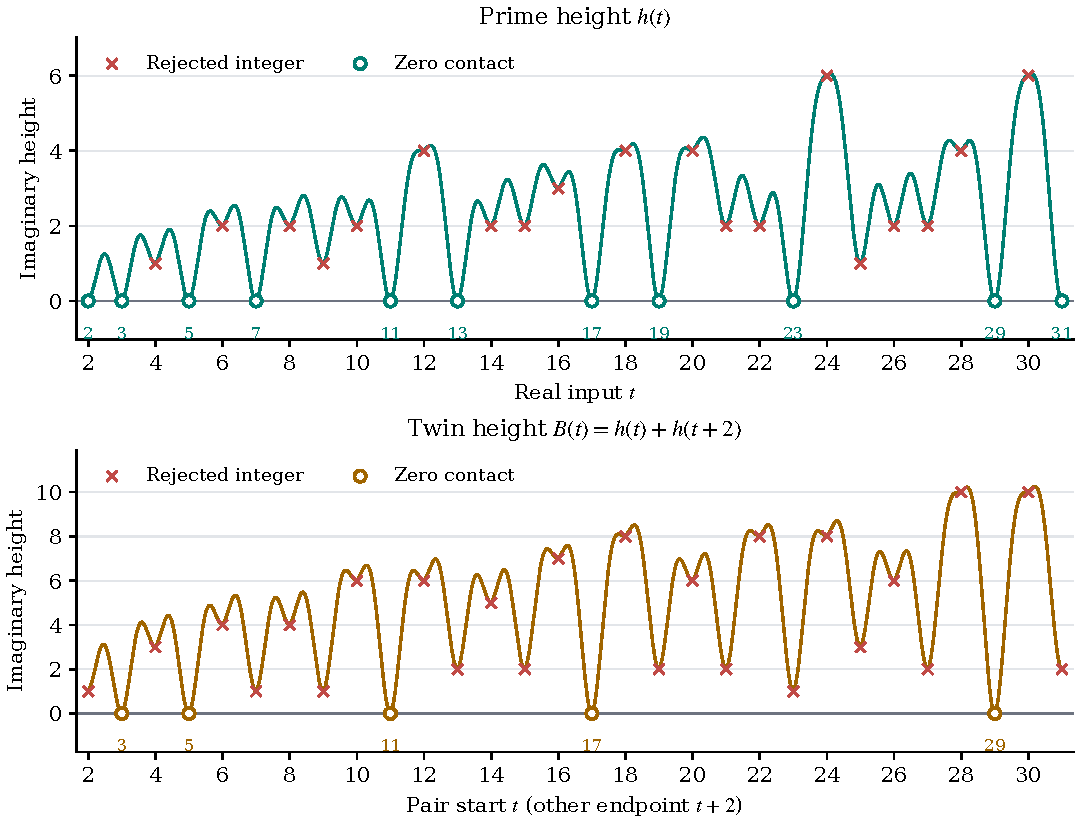
\includegraphics[width=\textwidth]{figures/prime-twin-contacts.pdf}
\caption{Prime and twin contacts. Completed curves use filters through $33$
on $[2,31]$. Circles are exact zero contacts and crosses are rejected integer
samples; the lower panel uses $t$ as the pair start and $t+2$ as the other
endpoint.}
\label{fig:prime-twin-contacts}
\end{figure}
